\documentclass[border=3pt]{standalone}
\usepackage{tikz}
\usetikzlibrary{decorations.pathreplacing,patterns}
\definecolor{greengreen}{rgb}{0.0, 0.42, 0.24}
%%%%%%%%%%%%%%%%%%%%%%%%%%%%%%%%%%%%%%%%%%%%%%%%%%%%%%%%%%%%%%%%%
\begin{document}
%%%%%%%%%%%%%%%%%%%%%%%%%%%%%%%%%%%%%%%%%%%%%%%%%%%%%%%%%%%%%%%%%
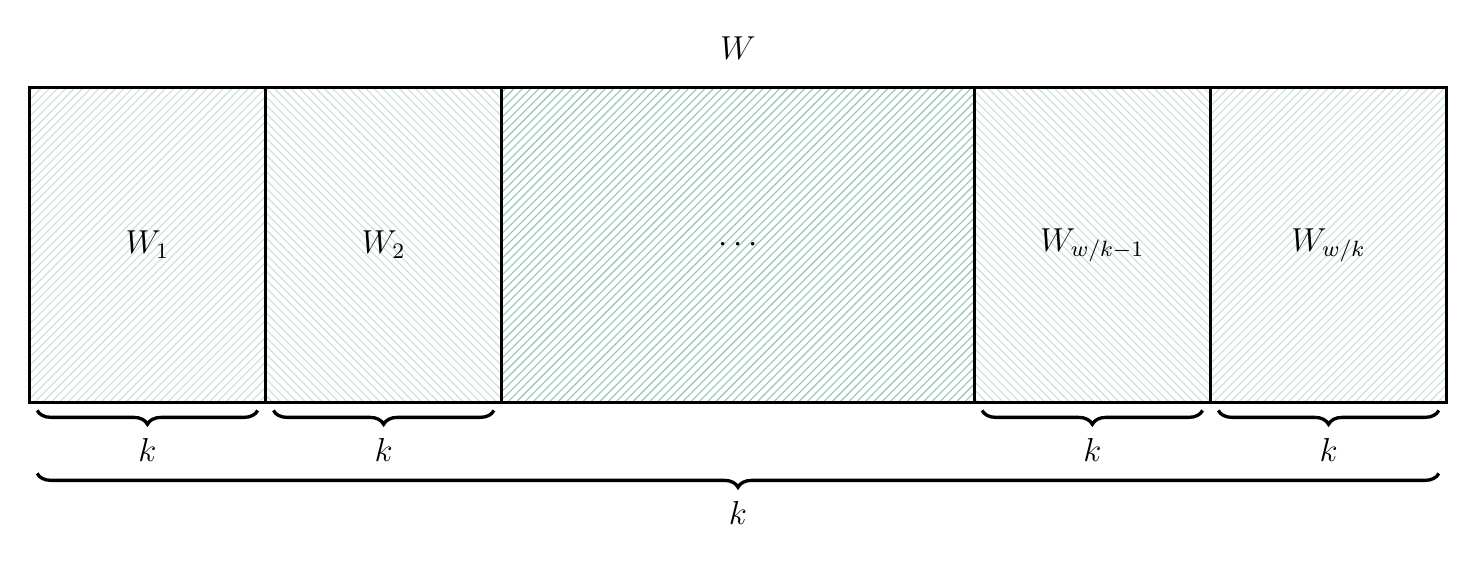
\begin{tikzpicture}[blue/.style={fill=blue,very thick,circle,inner sep=0pt}]
%================================================================
%	Boxes
\draw[very thick, pattern=north east lines, pattern color=greengreen!20] (0,0) rectangle (3,4); 
\draw[very thick, pattern=north west lines, pattern color=greengreen!20] (3,0) rectangle (6,4); 
\draw[very thick, pattern=north east lines, pattern color=greengreen!40] (6,0) rectangle (12,4); 
\draw[very thick, pattern=north west lines, pattern color=greengreen!20] (12,0) rectangle (15,4); 
\draw[very thick, pattern=north east lines, pattern color=greengreen!20] (15,0) rectangle (18,4);
%----------------------------------------------------------------
\node at (1.5,2) {\large $W_1$};
\node at (4.5,2) {\large $W_2$}; 
\node at (9,2) {\large $\cdots$}; 
\node at (13.5,2) {\large $W_{w/k-1}$}; 
\node at (16.5,2) {\large $W_{w/k}$}; 
%================================================================
%	Outside
\node at (9,4.5) {\large $W$};
\draw[very thick, decorate,decoration={brace,amplitude=5pt,mirror}] (0.1,-0.1) -- (2.9,-0.1);
\draw[very thick, decorate,decoration={brace,amplitude=5pt,mirror}] (3.1,-0.1) -- (5.9,-0.1);
\draw[very thick, decorate,decoration={brace,amplitude=5pt,mirror}] (12.1,-0.1) -- (14.9,-0.1);
\draw[very thick, decorate,decoration={brace,amplitude=5pt,mirror}] (15.1,-0.1) -- (17.9,-0.1);
%----------------------------------------------------------------
\node at (1.5,-0.6) {\large $k$};
\node at (4.5,-0.6) {\large $k$};
\node at (13.5,-0.6) {\large $k$};
\node at (16.5,-0.6) {\large $k$};
%----------------------------------------------------------------
\draw[very thick, decorate,decoration={brace,amplitude=5pt,mirror}] (0.1,-0.9) -- (17.9,-0.9);
\node at (9,-1.4) {\large $k$};

%================================================================
\end{tikzpicture}
%%%%%%%%%%%%%%%%%%%%%%%%%%%%%%%%%%%%%%%%%%%%%%%%%%%%%%%%%%%%%%%%%
\end{document}
%%%%%%%%%%%%%%%%%%%%%%%%%%%%%%%%%%%%%%%%%%%%%%%%%%%%%%%%%%%%%%%%%